\chapter{Neccessary Theoretical Background}\label{chap:theory}

\section{Introduction to Gaussian Processes}

This introduction is heavily inspired by \cite{rasmussen}.

A \acrfull{gp} can formally be defined as Definition \ref{def:gp}.

\newtheorem{gp_def}{Definition}
\begin{gp_def}\label{def:gp}
A Gaussian Process is a collection of random variables, any finite number of which has a joint Gaussian Distribution.
\end{gp_def}

In this thesis we will use a more specific definition in order to interpret \acrshort{gp}'s as a statistical distribution over functions. A \acrshort{gp} for a random function $f(\boldsymbol{x})$ is fully specified by its mean function $m(\boldsymbol{x})$ and covariance function $k(\boldsymbol{x}, \boldsymbol{x}')$.

\begin{equation}\label{eq:gp}
    f(\boldsymbol{x}) \sim GP(\;m(\boldsymbol{x}), \; k(\boldsymbol{x}, \boldsymbol{x}')\;)
\end{equation}

This interpretation of a \acrshort{gp} might seem a bit odd at first. The key observation is that the marginal distribution $p(\boldsymbol{x})$ of a multivariate Gaussian distribution $p(\boldsymbol{x}, \boldsymbol{y})$ is another Gaussian distribution that is completetly independet of $\boldsymbol{y}$, as expressed in \cref{eq:gaussian_marginal}. Any variables that is not of intereset can therefore easily be marginalized away, leaving only the subset of variables we care about.

\begin{equation}\label{eq:gaussian_marginal}
    p(\boldsymbol{x}) = \int_{\boldsymbol{y}} \mathcal{N} \bigg(\begin{bmatrix}
        \boldsymbol{x} \\ \boldsymbol{y}
    \end{bmatrix}\; \bigg| \begin{bmatrix}
        \boldsymbol{\mu_x} \\ \boldsymbol{\mu_y}
    \end{bmatrix}, \; \begin{bmatrix}
        \boldsymbol{\Sigma_{xx}} & \boldsymbol{\Sigma_{xy}} \\
        \boldsymbol{\Sigma_{yx}} & \boldsymbol{\Sigma_{yy}} \\
    \end{bmatrix} \bigg) d\boldsymbol{y} = \mathcal{N} \big( \boldsymbol{x} \;\big| \; \boldsymbol{\mu_x}, \boldsymbol{\Sigma_{xx}}\big)
\end{equation}

Any \acrshort{gp} by Definition \ref{def:gp} can therefore be thought of as the finite marginal distribution of an infinite Gaussian Distribution, jointly describing the values of $f(\boldsymbol{x})$ at all possible inputs $\boldsymbol{x}$. In the end, a \acrshort{gp} is nothing more than a joint Gaussian Distribution with a fancy interpretation.

\subsection{Conditioning}
So far, we have only specified the prior distribution over $f(\boldsymbol{x})$, and so far the \acrshort{gp}.  

\subsection{Introduction to kernels}
The covariance function $k(\boldsymbol{x}, \boldsymbol{x}')$ determines the similarity between two different points $\boldsymbol{x}$ and $\boldsymbol{x}'$. These covariance functions will in this theis be referred to as a \textit{kernel}, which maps the input space to a \textit{feature-space} \cite{rasmussen}. The key idea behind kernels is that the kernels may in many cases be simpler to compute than the input vectors themselves if the input-space is complex. The output of the kernel is a value describing the similarity (i.e. covariance) between the two inputs. Different types of kernels will be discussed in greater detail in \cref{sec:kernels}.

The kernel must be positive definite in order to produce a valid covariance matrix, which requires that

\begin{equation}
    k(\boldsymbol{x}, \boldsymbol{x}') = k(\boldsymbol{x}', \boldsymbol{x})
\end{equation}

The resulting covariance matrix $K(X, X)$ is the result of calling $k(\cdot, \cdot)$ on all pairs on inputs, i.e.
\begin{equation}
    K(X, X)_{ij} = k(\boldsymbol{x}_i, \boldsymbol{x}_j) \quad \forall i, j
\end{equation}

\subsection{Conditioning}
So far we have only specified the prior distribution for $f(\boldsymbol{x})$. 
As an example, we use the simple \acrshort{gp} in \cref{eq:theory_simple_gp}. The \acrshort{rbf} kernel used will be introduced in greater detail in \cref{sec:kernels_rbf}. The latent function $f(x)$ is the true relationship between $f$ and $x$, which can only be observed through the noisy observations $y_i$. 

\begin{align}\label{eq:theory_simple_gp}
    \begin{split}
    k(x, x') &= \exp\bigg(-\frac{|| x - x'||^2}{2}\bigg)\\
    f(x) &\sim \text{GP}(0, k(x, x'))\\
    y_i &= f(x_i) + \epsilon
    \end{split}
\end{align}

Before any observations are made we can only rely on prior information as shown in \cref{fig:gp_prior}. From a Bayesian perspective, we then want to observe values $y_i$ and update our prior beliefs to get the posterior distribution for $f(x)$.

\begin{figure}[h]
    \centering
    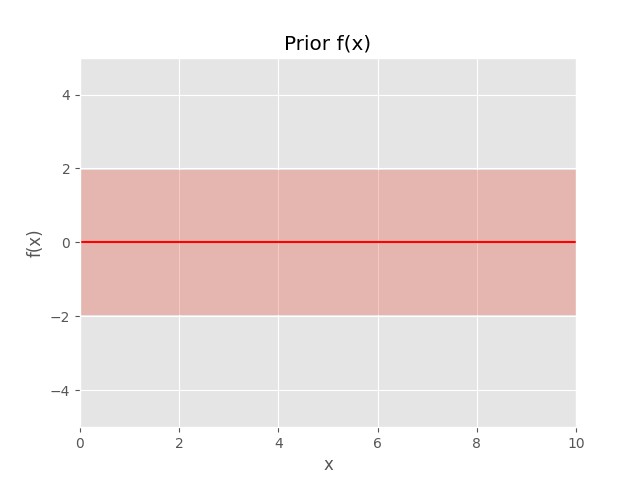
\includegraphics[width=0.8\textwidth]{figures/introduction-gp/prior.png}
    \caption{Gaussian Process Prior}
    \label{fig:gp_prior}
\end{figure}

\section{Model Selection}
\section{Kernels}\label{sec:kernels}

\subsection{Radial Basis Function}\label{sec:kernels_rbf}
\section{Multivariate Gaussian Process}
\section{Computational Complexity}
\section{Approximate methods}
\subsection{Variational Inference}
\subsection{Markov Chain Monte Carlo}
